% This is samplepaper.tex, a sample chapter demonstrating the
% LLNCS macro package for Springer Computer Science proceedings;
% Version 2.20 of 2017/10/04
%
\documentclass[runningheads]{llncs}
%
\usepackage{graphicx}
\graphicspath{ {./images/} }
\usepackage[utf8]{inputenc}
\usepackage[spanish,es-nodecimaldot]{babel}
\usepackage[spanish, fixlanguage]{babelbib}
% Used for displaying a sample figure. If possible, figure files should
% be included in EPS format.
%
% If you use the hyperref package, please uncomment the following line
% to display URLs in blue roman font according to Springer's eBook style:
% \renewcommand\UrlFont{\color{blue}\rmfamily}

\begin{document}
%
\title{Consejo de embajadores}
\subtitle{Una variación del Naming Game basado en comunidades}
%
%\titlerunning{Abbreviated paper title}
% If the paper title is too long for the running head, you can set
% an abbreviated paper title here
%
\author{Diego de Jesús Isla López \and
Saul Ivan Rivas Vega}
%
% First names are abbreviated in the running head.
% If there are more than two authors, 'et al.' is used.
%
\institute{Universidad Nacional Autónoma de México, Ciudad Universitaria, Ciudad de México, México\\
\email{\{diego.isla,saul.ivan.rivas.vega\}@comunidad.unam.mx}}
%
\maketitle              % typeset the header of the contribution
%
\begin{abstract}
El Naming Game es una simulación basada en agentes los cuales con un protocolo de comunicación y una memoria buscan llegar a un acuerdo sobre que única palabra almacenar para nombrar a un objeto. En el presente trabajo extendemos las características del diseño original propuesto por Baronchelli, con el propósito de reportar y analizar las diferencias en los parámetros de estudio durante la simulación. Se llevaron a cabo una serie de experimentos por cada combinación posible dentro de un espacio reducido de valores y la media de resultados son los tomados en cuenta para el análisis. Los resultados son congruentes con los reportes de Baronchelli, además de que se puede observar comportamientos especiales.
\keywords{Naming Game  \and Comunicación \and Agentes \and Inteligencia Artificial \and Simulación.}
\end{abstract}
%
%
%
\section {Introducción}
Se han realizado trabajos con experimentos basados en la hipótesis de que el lenguaje es un sistema adaptativo que se forma así mismo a través de un proceso cultural auto-organizado~\cite{ref_article1}.

Los juegos del lenguaje fueron propuestos por primera vez en las investigaciones filosóficas de Ludwig Wittgenstein en 1967~\cite{ref_article1}. Su modelo consiste en considerar a un constructor y a un asistente con distintas herramientas y recursos los cuales el constructor debía solicitar al asistente, lo cual llevaba a comunicarse en un lenguaje primitivo. Sin embargo, Wittgenstein no creía que así era como se comportaba el lenguaje en el mundo real. Lo que el pensaba era que podían reconocerse particularidades de la lingüística que si se asemejan al mundo real.

Posteriormente se realizaron implementaciones de variada complejidad como lo son: \textit{Naming Games}~\cite{ref_article1}, \textit{Guessing Games}~\cite{ref_article1}, \textit{Descripting Games}~\cite{ref_article1}, etc.
\section{Antecedentes}
El trabajo propuesto en Naming Games~\cite{ref_article1} inspiró el trabajo de Baronchelli~\cite{ref_article1} para desarrollar un modelo de comunicación entre agentes. En dicho modelo se utilizaba el siguiente protocolo de comunicación entre el hablante y el escucha que son 2 agentes seleccionados al azar:
\begin{itemize}
	\item El hablante selecciona un objeto del contexto actual
	\item El hablante toma una palabra de su inventario para referirse al objeto, en caso de no tener una palabra, crea una nueva.
	\item El hablante comunica la palabra seleccionada al receptor
	\item Si el escucha tiene en su inventario la palabra que le comunicó el hablante, la comunicación se considera exitosa lo que hace que tanto el hablante como el escucha borren su inventario de palabras para el objeto con excepción de la palabra que ambos conocen.
	\item En caso contrario el escucha almacena en su inventario de palabras la palabra que le comunicó el hablante.
\end{itemize}

\section{Diseño Propuesto}

La variante del \textit{naming game} propuesta consiste en tener comunidades con un número uniforme de miembros. Cada comunidad utiliza un conjunto de reglas para generar palabras diferentes con las cuales designarán a cada uno de los objetos. Cada comunidad decidirá la palabra que le asignará a cada objeto y una vez que todas han llegado a un consenso, los embajadores de cada comunidad se reúnen y entre todos presentan las palabras de sus comunidades y votan las palabras que usarán de ahora en adelante. Una vez que se deciden las palabras finales, los embajadores regresan a sus respectivas comunidades y enseñan las palabras a los demás miembros.

\subsection{Protocolos de comunicación}

Se tienen tres protocolos de comunicación uno por cada etapa del sistema:

\begin{enumerate}
	\item Comunicación entre miembros de una misma comunidad.
	\item Comunicación entre embajadores.
	\item Comunicación del embajador con el resto de su comunidad.
\end{enumerate}
\subsubsection{Primera Etapa}
\paragraph{Comunicación entre miembros de una comunidad}
En esta etapa del sistema las comunicaciones se realizan solamente entre miembros de una misma comunidad y termina hasta que todas las comunidades converjan internamente.
Se sigue el siguiente protocolo de comunicación:
\begin{enumerate}
	\item Tomar 1 comunidad aleatoriamente que no haya convergido internamente aún.
	\item Seleccionar aleatoriamente al agente que escucha y el agente que habla.
	\item Seleccionar el objeto aleatoriamente.
	\item Si el hablante no tiene palabras en su memoria, crea una con base en su regla de generación y la almacena con frecuencia = 1.
	\item El hablante toma la palabra con mayor frecuencia en su memoria.
	\item Si el escucha no conoce la palabra la almacena con una frecuencia = 1.
	\item Si el escucha si conoce la palabra aumenta en 1 su frecuencia y reduce por un factor de olvido (16, suelo) las demás palabras en su memoria.
	\item Si alguna palabra llega a 0 se elimina de su memoria. 
\end{enumerate}

\subsubsection{Segunda Etapa}
En esta etapa del sistema las comunicaciones se realizan solamente entre los embajadores. Existe exactamente un embajador por comunidad, y este puede ser cualquier miembro de la comunidad puesto que todos terminaron con la misma lista de palabras. Comienzan las comunicaciones al finalizar la etapa anterior y terminan hasta que todos los embajadores conozcan la palabra de los demás embajadores.
Se sigue el siguiente protocolo de comunicación:
\begin{enumerate}
	\item El embajador de cada comunidad puede ser cualquiera, se toma al primero de cada comunidad.
	\item Se fuerza la comunicación de todos los embajadores como hablante con cada uno de los otros embajadores como escuchas con cada uno de los objetos.
	\item En cada una de las comunicaciones el embajador hablante comunica la única palabra que tiene actualmente en su memoria.
	\item El escucha evalúa la preferencia por la nueva palabra y si la prefiere en lugar de su palabra actual, la reemplaza, y en caso contrario, la ignora.
	\item Posterior a que todos los embajadores se hayan comunicado y escogieran su palabra preferida, vuelven a comunicarse entre todos.
	\item El hablante escoge su palabra que seleccionó como favorita.
	\item Si el escucha si conoce la palabra aumenta en 1 su frecuencia, en caso contrario la agrega con frecuencia = 1.
	\item Todos los embajadores borran todas las palabras de su memoria, con excepción de la palabra más frecuente en el consejo.
\end{enumerate}
\subsubsection{Tercera Etapa}
Esta es la etapa final del sistema en la que solamente los embajadores propagan la lista de palabras que se obtuvo del consejo y los agentes dentro de la comunidad solo reemplazan la lista que tenían con la del embajador. Las comunicaciones solo se llevan a cabo con el embajador como el hablante y los demás agentes de su comunidad como oyentes. Terminan las comunicaciones cuando todos los agentes de todas las comunidades terminan con la misma lista de palabras.
Se sigue el siguiente protocolo de comunicación:
\begin{enumerate}
	\item El embajador de cada comunidad Comunica su palabra de cada objeto a un miembro de su comunidad con quien no se haya comunicado aún.
	\item El escucha reemplaza la palabra para cada objeto con la que le comunica el embajador.
\end{enumerate}

\subsection{Generación de palabras}
Existe un diccionario inicial de sílabas tomadas a partir de concatenar las vocales con cada una de las consonantes del alfabeto. Una \textit{regla de generación} consiste en una tupla $(A,cantidad\_s,separador)$ en donde $A$ es un subconjunto del diccionario de sílabas, $cantidad\_s$ es un entero positivo que determina la cantidad de sílabas que se usarán para formar la palabra y el $separador$ es un elemento del diccionario el cual se coloca entre cada silaba que formó a la palabra.

Se tiene un conjunto de cuatro reglas de generación de palabras. 


\subsection{Evaluación de preferencia}

Entre embajadadores, se evalúa la preferencia al recibir una palabra de una comunidad ajena. Esto se hace comparando la palabra recibida con respecto a las reglas de generación del receptor. Por el momento se hace una evaluación simple que favorece la elección de palabras muy largas.
\subsection{Convergencia}


\section{Experimentos}


Descripción de las distintas combinaciones.
\section{Resultados}
\section{Discusión y Conclusiones}
\section{Introducción}
\subsection{A Subsection Sample}Please note that the first paragraph of a section or subsection is
not indented. The first paragraph that follows a table, figure,
equation etc. does not need an indent, either.

Subsequent paragraphs, however, are indented.

\subsubsection{Sample Heading (Third Level)} Only two levels of
headings should be numbered. Lower level headings remain unnumbered;
they are formatted as run-in headings.

\paragraph{Sample Heading (Fourth Level)}
The contribution should contain no more than four levels of
headings. Table~\ref{tab1} gives a summary of all heading levels.

\begin{table}
\caption{Table captions should be placed above the
tables.}\label{tab1}
\begin{tabular}{|l|l|l|}
\hline
Heading level &  Example & Font size and style\\
\hline
Title (centered) &  {\Large\bfseries Lecture Notes} & 14 point, bold\\
1st-level heading &  {\large\bfseries 1 Introduction} & 12 point, bold\\
2nd-level heading & {\bfseries 2.1 Printing Area} & 10 point, bold\\
3rd-level heading & {\bfseries Run-in Heading in Bold.} Text follows & 10 point, bold\\
4th-level heading & {\itshape Lowest Level Heading.} Text follows & 10 point, italic\\
\hline
\end{tabular}
\end{table}


\noindent Displayed equations are centered and set on a separate
line.
\begin{equation}
x + y = z
\end{equation}
Please try to avoid rasterized images for line-art diagrams and
schemas. Whenever possible, use vector graphics instead (see
Fig.~\ref{fig1}).

\begin{figure}
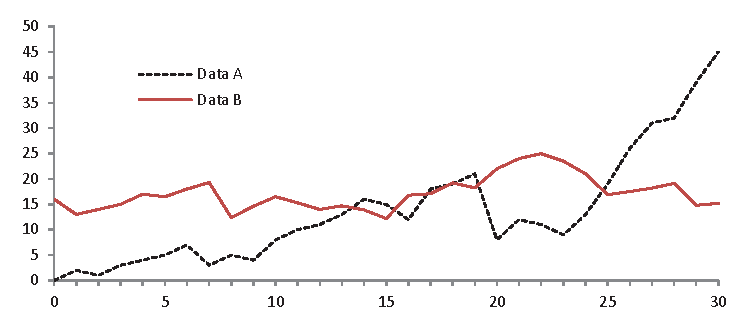
\includegraphics[width=\textwidth]{fig1.eps}
\caption{A figure caption is always placed below the illustration.
Please note that short captions are centered, while long ones are
justified by the macro package automatically.} \label{fig1}
\end{figure}

\begin{theorem}
This is a sample theorem. The run-in heading is set in bold, while
the following text appears in italics. Definitions, lemmas,
propositions, and corollaries are styled the same way.
\end{theorem}
%
% the environments 'definition', 'lemma', 'proposition', 'corollary',
% 'remark', and 'example' are defined in the LLNCS documentclass as well.
%
\begin{proof}
Proofs, examples, and remarks have the initial word in italics,
while the following text appears in normal font.
\end{proof}
For citations of references, we prefer the use of square brackets
and consecutive numbers. Citations using labels or the author/year
convention are also acceptable. The following bibliography provides
a sample reference list with entries for journal
articles~\cite{ref_article1}, an LNCS chapter~\cite{ref_lncs1}, a
book~\cite{ref_book1}, proceedings without editors~\cite{ref_proc1},
and a homepage~\cite{ref_url1}. Multiple citations are grouped
\cite{ref_article1,ref_lncs1,ref_book1},
\cite{ref_article1,ref_book1,ref_proc1,ref_url1}.
%
% ---- Bibliography ----
%
% BibTeX users should specify bibliography style 'splncs04'.
% References will then be sorted and formatted in the correct style.
%
% \bibliographystyle{splncs04}
% \bibliography{mybibliography}
%
\begin{thebibliography}{8}
\bibitem{ref_article1}
Author, F.: Article title. Journal \textbf{2}(5), 99--110 (2016)

\bibitem{ref_lncs1}
Author, F., Author, S.: Title of a proceedings paper. In: Editor,
F., Editor, S. (eds.) CONFERENCE 2016, LNCS, vol. 9999, pp. 1--13.
Springer, Heidelberg (2016). \doi{10.10007/1234567890}

\bibitem{ref_book1}
Author, F., Author, S., Author, T.: Book title. 2nd edn. Publisher,
Location (1999)

\bibitem{ref_proc1}
Author, A.-B.: Contribution title. In: 9th International Proceedings
on Proceedings, pp. 1--2. Publisher, Location (2010)

\bibitem{ref_url1}
LNCS Homepage, \url{http://www.springer.com/lncs}. Last accessed 4
Oct 2017
\end{thebibliography}
\end{document}
